\chapter{Amplificador de Bajo Ruido (LNA)}
\label{chap:lna}

Este capítulo presenta el diseño y simulación del Amplificador de Bajo Ruido (LNA) del radar FMCW.

\section{Introducción Teórica}
La etapa de Amplificador de Bajo Ruido (Low Noise Amplifier, LNA) constituye uno de los bloques más críticos dentro de la cadena de recepción del radar, ya que determina en gran medida el piso de ruido total del sistema. Esta afirmación se fundamenta en la fórmula de Friis para la figura de ruido total de una cadena de amplificación, que establece que el ruido global está dominado principalmente por la primera etapa activa que aporta ganancia:

\[
F_T = F_1 + \frac{F_2 - 1}{A_1} + \frac{F_3 - 1}{A_1 A_2} + \cdots
\]
De esta expresión se desprende que una baja figura de ruido y una ganancia adecuada en la primera etapa resultan determinantes para el desempeño global del receptor. En consecuencia, el diseño del LNA se orienta a minimizar la figura de ruido, manteniendo simultáneamente niveles aceptables de ganancia, estabilidad y linealidad.

\section{Topología adoptada y circuito de referencia}
Para la implementación del LNA se tomó como referencia el circuito propuesto por NXP en la nota de aplicación AN11426, el cual utiliza el transistor bipolar de bajo ruido BFU550W. Dicho transistor está específicamente diseñado para aplicaciones de radiofrecuencia en el rango de cientos de MHz hasta algunos GHz, priorizando un bajo ruido intrínseco.

El circuito de la AN11426 emplea una configuración de emisor común con polarización fija. Esta topología permite obtener una elevada ganancia de potencia, a costa de una mayor sensibilidad frente a variaciones de temperatura y dispersión de parámetros del transistor. No obstante, resulta adecuada para aplicaciones académicas y de laboratorio, donde dichas variaciones pueden ser controladas o compensadas.

Según el fabricante, el circuito propuesto es capaz de cumplir con los siguientes requerimientos típicos:
Tensión de alimentación: 
\begin{itemize}
\item \textbf{Corriente de colector}: $20\,\text{mA}$ (a temperatura ambiente)
\item \textbf{Figura de ruido}: $NF<1.4\,\text{dB}$
\item \textbf{Ganancia de potencia}: aproximadamente $12\,\text{dB}$
\item \textbf{Return Loss de entrada}: menor a $-8\,\text{dB}$
\item \textbf{Return Loss de salida}: menor a $-10\,\text{dB}$
\end{itemize}

\begin{figure}[htbp]
\centering
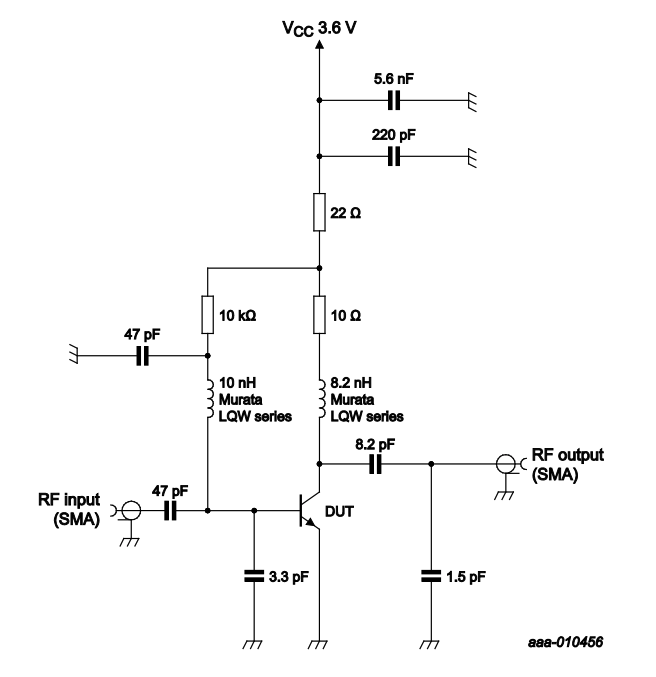
\includegraphics[width=0.6\textwidth]{Figures/LNA/AN11426_reference.png}
\captionsetup{justification=centering}
\caption{Circuito propuesto por NXP en su \\ nota de aplicación AN11426}
\end{figure}

\newpage
\section{Simulación}
\subsection{Punto de polarizacion:}

El BFU550W es un transistor bipolar de bajo ruido, orientado a aplicaciones de RF donde la figura de ruido es un parámetro crítico. Si bien actualmente se encuentra discontinuado, continúa siendo una referencia válida desde el punto de vista didáctico.

\begin{figure}[htbp]
\centering
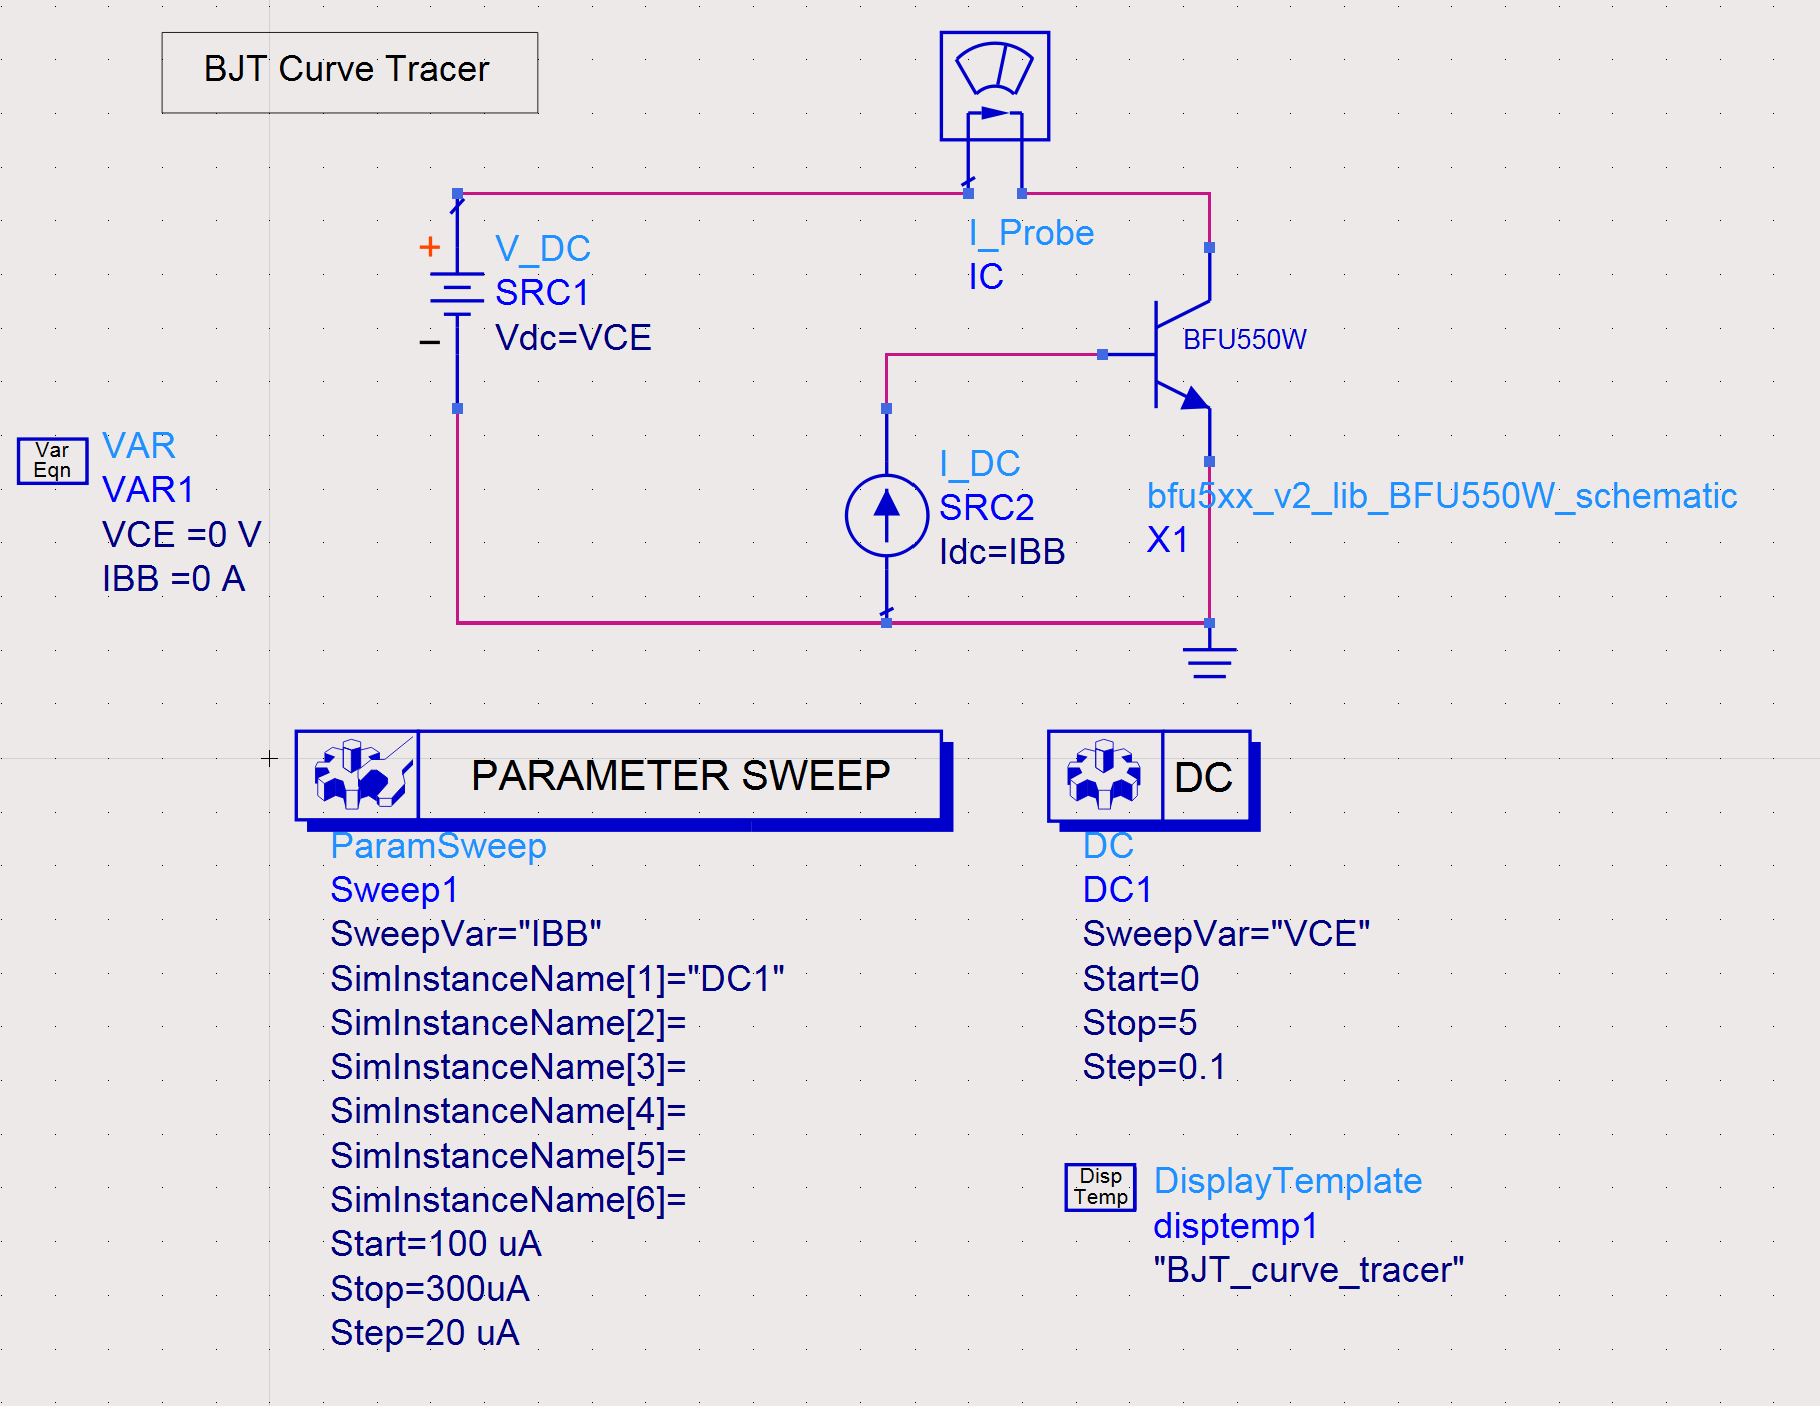
\includegraphics[width=0.65\textwidth]{Figures/LNA/BFU550W_Vce_VS_Ic.png}
\captionsetup{justification=centering}
\caption{Template BJT\_curve\_tracer utilizando el transistor BFU550W,\\ se encuentra en LNA/BFU550W\_Vce\_VS\_Ic}
\end{figure}

\begin{figure}[htbp]
\centering
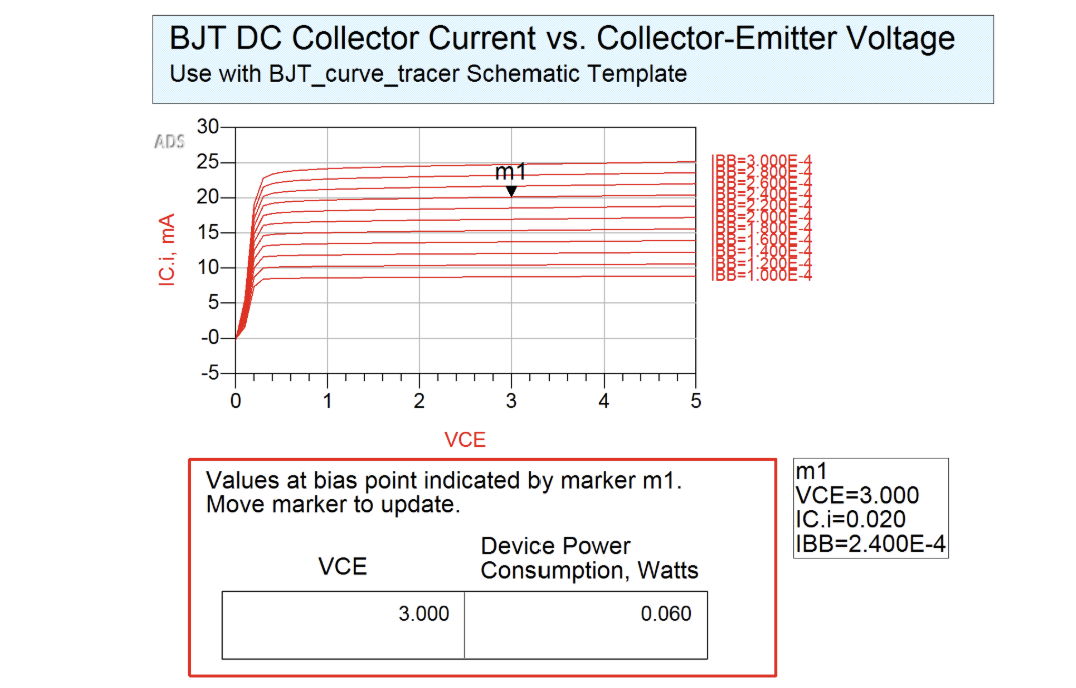
\includegraphics[width=0.65\textwidth]{Figures/LNA/BFU550W_Vce_VS_Ic_resultado.png}
\captionsetup{justification=centering}
\caption{Curvas características Ic vs Vce del \\transistor BFU550W
obtenidas mediante el test bench}
\end{figure}

Para el análisis del punto de polarización se utilizó el software ADS, fijando una corriente de colector de $20\,\text{mA}$ y obteniendo una tensión colector–emisor cercana a $3\,\text{V}$. Se eligió esta punto de polarización debido a que fue el seleccionado en la nota de aplicacion AN11426 en la cual se busco un muy bajo ruido con una buena ganancia. El análisis DC se realizó mediante un template específico de ADS, que permite evaluar las características estáticas del transistor en función de la corriente y la tensión aplicadas. Tambien se grafico la $NF_{min}$ la cual seria el piso de ruido que nos daria el transistor configurado con una $V_{CE}=3\,\text{V}$ y una $I_C=20\,\text{mA}$. Esta figura de ruido limitara el piso de ruido que puede tener el LNA.



\begin{figure}[htbp]
\centering
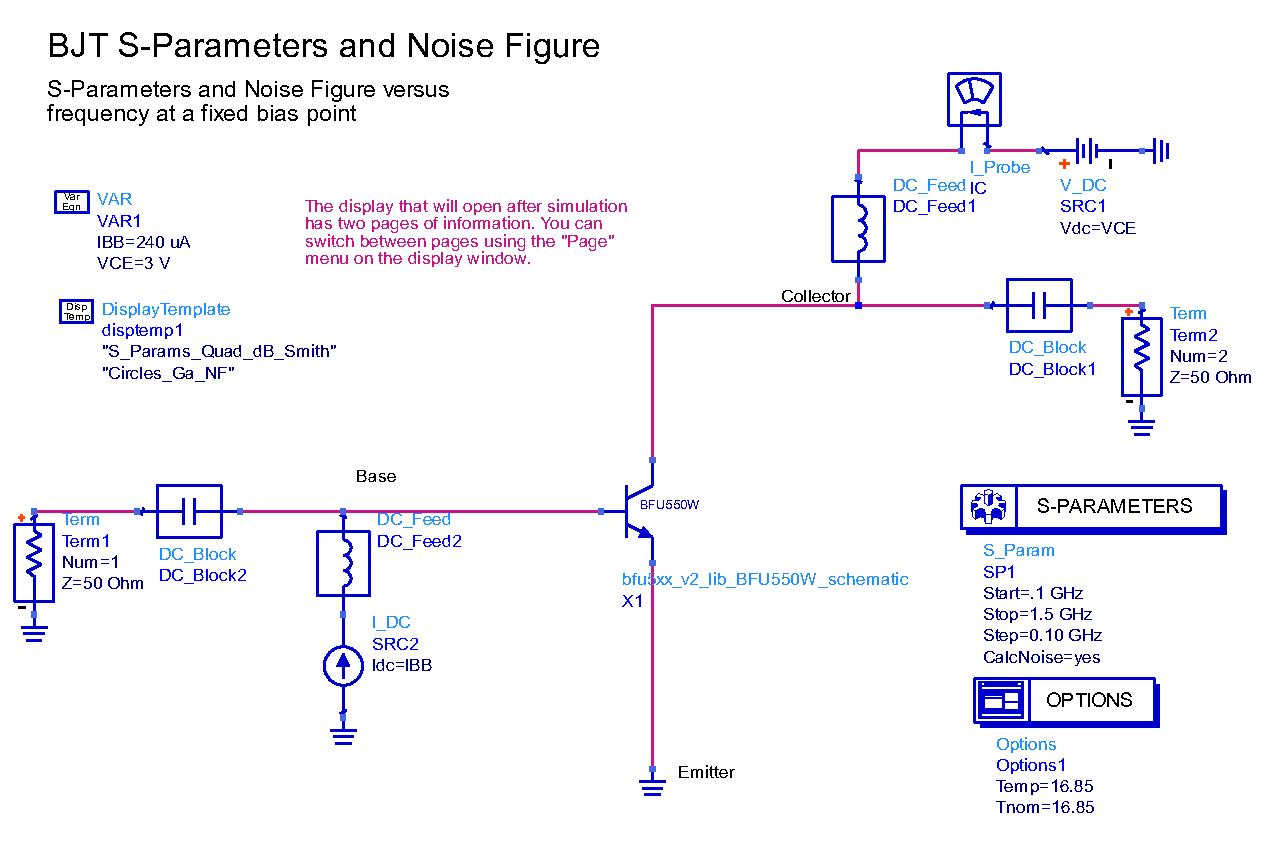
\includegraphics[width=0.65\textwidth]{Figures/LNA/lna_bfu_curves_schematic.pdf}
\captionsetup{justification=centering}
\caption{Template BJT S-Parameters and Noise Figure utilizando BFU550W \\se encuentra en LNA/BFU550W\_Noise}
\end{figure}

\begin{figure}[htbp]
\centering
\begin{tikzpicture}
\begin{axis}[
    width=0.95\textwidth,
    height=7cm,
    xlabel={Frecuencia [GHz]},
    ylabel={Noise Figure},
    grid=both,
    grid style={line width=.1pt, draw=gray!30},
    major grid style={line width=.2pt, draw=gray!50},
    tick label style={font=\footnotesize},
    label style={font=\small},
    legend style={font=\small, at={(0.02,0.98)}, anchor=north west},
]

% nf[2]
\addplot[blue, thick]
table[x expr=\thisrowno{3}/1e9, y index=1] {Datasets/5_LNA/noise_alone.dat};
\addlegendentry{nf[2]}

% NFmin
\addplot[green!60!black, thick]
table[x expr=\thisrowno{3}/1e9, y index=2] {Datasets/5_LNA/noise_alone.dat};
\addlegendentry{$NF_\mathrm{min}$}

% ----- Cuadro informativo -----
\node[
    draw,
    fill=white,
    align=left,
    font=\footnotesize,
    anchor=north west
] at (rel axis cs:0.65,0.95) {
\textbf{En $1\,\text{GHz}$} \\[2pt]
nf[2] = 1.55 \\
$NF_\mathrm{min}$ = 0.949
};

\end{axis}
\end{tikzpicture}
\caption{Noise Figure en función de la frecuencia}
\label{fig:nf_vs_freq}
\end{figure}

Para el gráfico de $NF_{min}$ se utilizo otro template de ADS. Este template nos permitió observar el piso de ruido que tendríamos debido a la utilización del BFU550W evaluado con una tensión de colector emisor de $3\,\text{V}$ y una corriente de colector de $20\,\text{mA}$.



\subsection{Ganancia:}
La ganancia del amplificador se evaluó a partir del parámetro de dispersión $S_{21}$, que relaciona la onda incidente en la entrada con la onda transmitida hacia la carga. Según la información del fabricante, el transistor BFU550W puede alcanzar una ganancia máxima de aproximadamente $18\,\text{dB}$ para una corriente de colector de $20\,\text{mA}$.

En las simulaciones realizadas se obtuvo una ganancia máxima cercana a $15{,}5\,\text{dB}$ alrededor de $430\,\text{MHz}$, mientras que a $1\,\text{GHz}$ la ganancia se reduce a aproximadamente $13\,\text{dB}$. Este comportamiento es consistente con la respuesta en frecuencia del dispositivo y con la adaptación implementada en el circuito. En la Figura \ref{fig:lna_stage_schematic} se muestra el esquemático de la etapa LNA utilizado para las simulaciones.

\begin{figure}[htbp]
\centering
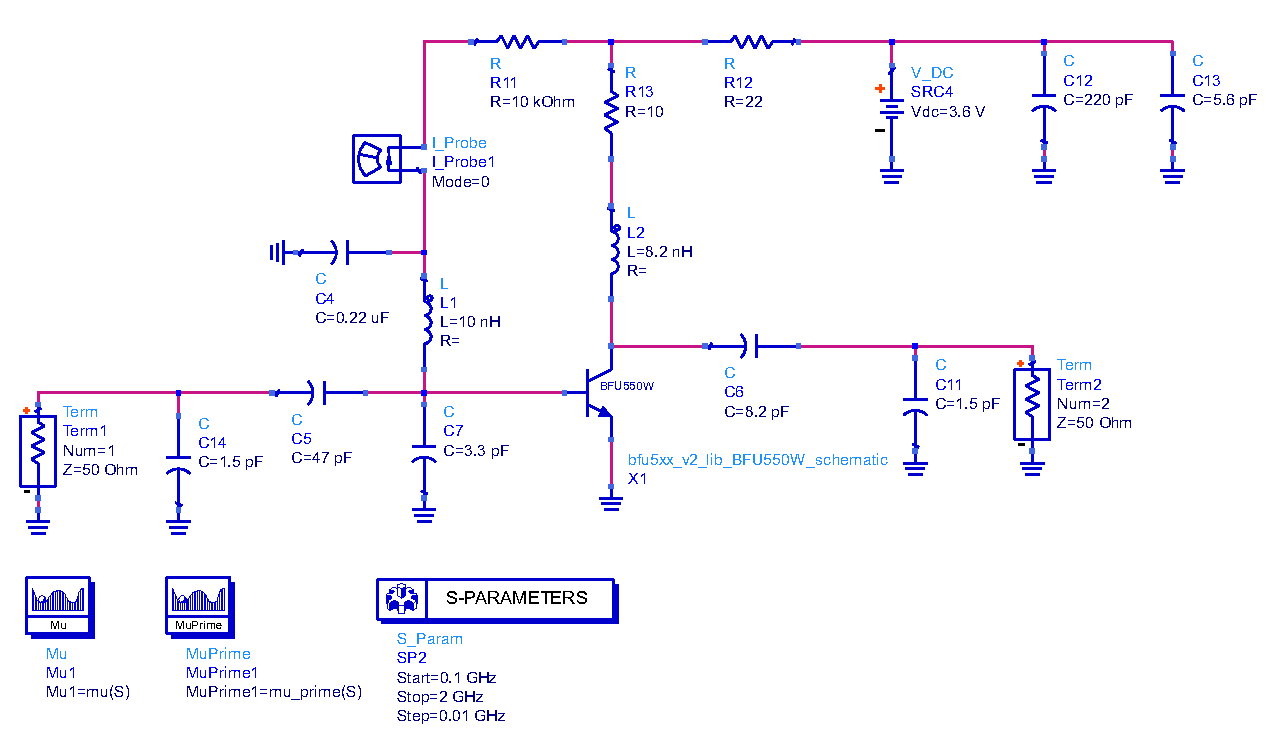
\includegraphics[width=0.85\textwidth]{Figures/LNA/lna_stage_schematic.pdf}
\captionsetup{justification=centering}
\caption{Esquemático de la etapa LNA utilizado para las simulaciones}
\label{fig:lna_stage_schematic}
\end{figure}


\begin{figure}[htbp]
\centering
\begin{tikzpicture}
\begin{axis}[
    width=0.95\textwidth,
    height=7cm,
    xlabel={Frecuencia [GHz]},
    ylabel={dB(S(2,1))},
    grid=both,
    grid style={line width=.1pt, draw=gray!30},
    major grid style={line width=.2pt, draw=gray!50},
    tick label style={font=\footnotesize},
    label style={font=\small},
    legend style={font=\small, at={(0.02,0.98)}, anchor=north west},
]

% nf[2]
\addplot[blue, thick]
table[x expr=\thisrowno{0}/1e9, y index=1] {Datasets/5_LNA/parametro_S21.dat};

\end{axis}
\end{tikzpicture}
\caption{Ganancia del circuito propuesto en la nota de aplicacion AN11426}
\label{fig:nf_vs_freq}
\end{figure}


\subsection{Figura de ruido:}
La figura de ruido es uno de los parámetros más relevantes en el diseño del LNA, ya que impacta directamente en la sensibilidad del receptor. La mínima figura de ruido alcanzable está limitada por las características intrínsecas del transistor y por el punto de polarización seleccionado.

Inicialmente se analizó la figura de ruido mínima  considerando únicamente el transistor, en un sistema ideal. En estas simulaciones se observan que la figura de ruido del BFU550W presenta un valor menor a $1\,\text{dB}$ en todo el rango a utilizar. Sin embargo, al incorporar nuestro
una carga de $50\,\Omega$ resulta necesaria una red de adaptación, lo que inevitablemente introduce un incremento en la figura de ruido total.

\begin{figure}[htbp]
\centering
\begin{tikzpicture}
\begin{axis}[
    width=0.95\textwidth,
    height=7cm,
    xlabel={Frecuencia [GHz]},
    ylabel={Noise Figure},
    grid=both,
    grid style={line width=.1pt, draw=gray!30},
    major grid style={line width=.2pt, draw=gray!50},
    tick label style={font=\footnotesize},
    label style={font=\small},
    legend style={font=\small, at={(0.02,0.98)}, anchor=north west},
]

% nf[2]
\addplot[blue, thick]
table[x expr=\thisrowno{3}/1e9, y index=1] {Datasets/5_LNA/ruido_AN11426.dat};
\addlegendentry{nf[2]}

% NFmin
\addplot[green!60!black, thick]
table[x expr=\thisrowno{3}/1e9, y index=2] {Datasets/5_LNA/ruido_AN11426.dat};
\addlegendentry{$NF_\mathrm{min}$}

% ----- Cuadro informativo -----
\node[
    draw,
    fill=white,
    align=left,
    font=\footnotesize,
    anchor=north west
] at (rel axis cs:0.65,0.95) {
\textbf{En $1\,\text{GHz}$} \\[2pt]
nf[2] = 1.52 \\
$NF_\mathrm{min}$ = 1.02
};

\end{axis}
\end{tikzpicture}
\caption{Noise Figure en función de la frecuencia}
\label{fig:nf_vs_freq}
\end{figure}

Al analizar el circuito completo se observó un aumento de la figura de ruido a bajas frecuencias, atribuible principalmente a una polarización no óptima para minimizar el ruido en ese rango. Asimismo, se verificó que la figura de ruido depende no solo de la frecuencia, sino también de la corriente de colector, la tensión  y la temperatura, lo que explica las diferencias observadas entre distintas simulaciones.


\subsection{Estabilidad:}
La estabilidad del amplificador se evaluó mediante los factores $\mu$ y $\mu'$, que permiten determinar si el circuito es incondicionalmente estable en todo el rango de frecuencias de interés. Para que el amplificador sea estable, ambos parámetros deben ser mayores que 1.


\begin{figure}[htbp]
\centering
\begin{tikzpicture}
\begin{axis}[
    width=0.95\textwidth,
    height=7cm,
    xlabel={Frecuencia [GHz]},
    ylabel={Estabilidad $\mu$},
    grid=both,
    grid style={line width=.1pt, draw=gray!30},
    major grid style={line width=.2pt, draw=gray!50},
    tick label style={font=\footnotesize},
    label style={font=\small},
    legend style={font=\small, at={(0.98,0.98)}, anchor=north east},
]

% nf[2]
\addplot[blue, thick]
table[x expr=\thisrowno{2}/1e9, y index=0] {Datasets/5_LNA/mu_AN11426.dat};
\addlegendentry{Mu1}

% NFmin
\addplot[green!60!black, thick]
table[x expr=\thisrowno{2}/1e9, y index=1] {Datasets/5_LNA/mu_AN11426.dat};
\addlegendentry{MuPrime1}

\end{axis}
\end{tikzpicture}
\caption{Estabilidad obtenida del circuito propuesto en AN11426}
\label{fig:nf_vs_freq}
\end{figure}

En las simulaciones se observó que el circuito cumple con la condición de estabilidad en el rango de operación, aunque se encuentra próximo a la inestabilidad a bajas frecuencias. Por este motivo, el diseño final contempla la posibilidad de incorporar componentes adicionales (capacitores y una resistencia) con el objetivo de mejorar el margen de estabilidad en una implementación práctica.


\subsection{Punto de compresión de $1\,\text{dB}$ (P1dB):}
El punto de compresión de $1\,\text{dB}$ es un parámetro fundamental para caracterizar los límites de operación lineal del LNA. Se define como el nivel de potencia de entrada para el cual la ganancia del amplificador se reduce en $1\,\text{dB}$ respecto de la ganancia obtenida en régimen lineal.


\begin{figure}[htbp]
\centering
\begin{tikzpicture}
\begin{axis}[
    width=0.95\textwidth,
    height=7cm,
    xlabel={Potencia de entrada [dBm]},
    ylabel={Potencia en la salida [dBm]},
    grid=both,
    grid style={line width=.1pt, draw=gray!30},
    major grid style={line width=.2pt, draw=gray!50},
    tick label style={font=\footnotesize},
    label style={font=\small},
    legend style={font=\small, at={(0.02,0.98)}, anchor=north west},
]

\addplot[blue, thick]
table[x index=0, y index=1] {Datasets/5_LNA/power_AN11426.dat};


\end{axis}
\end{tikzpicture}
\caption{Punto de compresión del circuito propuesto en AN11426}
\label{fig:nf_vs_freq}
\end{figure}




A bajas potencias de entrada, la relación entre la potencia de entrada y la potencia de salida es aproximadamente lineal. Sin embargo, al incrementar la potencia, el dispositivo comienza a operar en una región no lineal, produciéndose una saturación parcial. En las simulaciones se observó que este fenómeno comienza a manifestarse para potencias de entrada del orden de $-3\,\text{dBm}$.

Este efecto es mas visible en el siguiente gráfico en el cual la ganancia permanece constante hasta que comienza a disminuir debido a este efecto.

\begin{figure}[htbp]
\centering
\begin{tikzpicture}
\begin{axis}[
    width=0.95\textwidth,
    height=7cm,
    xlabel={Potencia de entrada [dBm]},
    ylabel={Ganancia},
    grid=both,
    grid style={line width=.1pt, draw=gray!30},
    major grid style={line width=.2pt, draw=gray!50},
    tick label style={font=\footnotesize},
    label style={font=\small},
    legend style={font=\small, at={(0.02,0.98)}, anchor=north west},
]

\addplot[blue, thick]
table[x index=0, y index=4] {Datasets/5_LNA/power_AN11426_nor.dat};
\addlegendentry{$Vout_1-Vin$}

\end{axis}
\end{tikzpicture}
\caption{Punto de compresión del circuito propuesto en AN11426
con la ganancia normalizada}
\label{fig:nf_vs_freq}
\end{figure}


\subsection{Productos de interpolación de tercer orden (IMD3):}
Debido a la naturaleza no lineal de los transistores bipolares, la excitación con señales de múltiples tonos genera componentes espectrales adicionales en la salida. En particular, los productos de interpolación de tercer orden (IMD3) resultan críticos en dispositivos bipolares debido a que suelen tener una amplitud mayor al resto de los armónicos.

\begin{figure}[htbp]
\centering
\begin{tikzpicture}
\begin{axis}[
    width=0.95\textwidth,
    height=7cm,
    xlabel={Potencia de entrada [dBm]},
    ylabel={Potencia en la salida [dBm]},
    grid=both,
    grid style={line width=.1pt, draw=gray!30},
    major grid style={line width=.2pt, draw=gray!50},
    tick label style={font=\footnotesize},
    label style={font=\small},
    legend style={font=\small, at={(0.02,0.98)}, anchor=north west},
]

\addplot[blue, thick]
table[x index=0, y index=1] {Datasets/5_LNA/power_AN11426.dat};
\addlegendentry{$dB(Fundamental)$}

\addplot[green, thick]
table[x index=0, y index=2] {Datasets/5_LNA/power_AN11426.dat};
\addlegendentry{$dB(Armonico_2)$}

\addplot[red, thick]
table[x index=0, y index=3] {Datasets/5_LNA/power_AN11426.dat};
\addlegendentry{$dB(Armonico_3)$}

\end{axis}
\end{tikzpicture}
\caption{Evolucion de la potencia del segundo y tercer armonico en el circuito propuesto en AN11426}
\label{fig:nf_vs_freq}
\end{figure}

Como se puede observar en el gráfico superior la potencia de la fundamental respecto a sus armónicos para bajas potencias de entrada es varios ordenes de magnitud mayor, sin embargo al acercar al punto de compresión la potencia de los armónicos se vuelven comparables.

\section{Resultados}

Como se pudo observar en este análisis, se obtuvo un bajo nivel de ruido junto con una ganancia adecuada, teniendo una figura de ruido menor a $1{,}5\,\text{dB}$ y una ganancia de $13\,\text{dB}$ en nuestra frecuencia de trabajo. Sin embargo, los resultados obtenidos difieren levemente de los presentados en la nota de aplicación, a pesar de que en ambos casos se utilizaron los mismos componentes.

En particular, nuestro análisis arrojó una figura de ruido aproximadamente $1\,\text{dB}$ mayor y una ganancia inferior, la cual no se encuentra centrada en el punto de interés. No obstante, la ganancia obtenida en nuestras simulaciones sigue siendo buena en nuestra frecuencia de trabajo.

A través de distintas simulaciones se intentó optimizar el diseño para aproximarlo más al propuesto en la nota de aplicación AN11426; sin embargo, no fue posible alcanzar resultados equivalentes.